\documentclass[uplatex,dvipdfmx]{jlreq}

\renewcommand{\baselinestretch}{1.1}
\setlength{\textwidth}{16cm}
\setlength{\textheight}{24cm}
\setlength{\evensidemargin}{0cm}
\setlength{\oddsidemargin}{0cm}
\setlength{\topmargin}{-1.0cm}

\usepackage[fleqn,tbtags]{mathtools}
\usepackage{listings,jvlisting}
\usepackage{jlreq-deluxe}
\usepackage[noalphabet]{pxchfon}
\usepackage{stix2}
\usepackage{hyperref}
\usepackage{here}
\usepackage{url}
\usepackage{comment}
\usepackage{bm}
\usepackage{ascmac}
\usepackage{tcolorbox}
\tcbuselibrary{breakable}
\usepackage{caption}

\captionsetup{format=hang}
\lstset{
  basicstyle={\ttfamily\small},
  identifierstyle={\small},
  commentstyle={\small\itshape\color{gray}},
  keywordstyle={\small\bfseries\color{blue}},
  stringstyle={\small\ttfamily\color{brown}},
  showstringspaces=false,
  frame={tb},
  breaklines=true,
  columns=[l]{fullflexible},
  numbers=left,
  numberstyle={\scriptsize},
  stepnumber=1,
  numbersep=1zw,
  lineskip=-0.5ex
}
\renewcommand{\lstlistingname}{ソースコード}
\newcounter{aibox}

\begin{document}

\title{ハッカソン1 第10週目 作業ログ \\ I2C同期を用いた輪唱曲演奏システム}
\author{7班 25G1035 金子稜侑}
%\date{}
\maketitle

\section{進捗要約}
\label{begin}

\ref{tasks}は，前回授業から今回授業までの，計画書およびWBSを元にした私の担当作業タスク一覧である．

\begin{tcolorbox}[title = 担当作業タスク一覧, arc=3mm, colback=white, breakable]
    \label{tasks}
     （A） 全体結合テストの実施：班員より共有された\texttt{week10/ptypes}を用いて，
     全Slave（ピアノ・フルート・木琴・ドラム）を接続した状態での演奏システムおよびクマアニメーションの合同動作確認を実施した．
     演奏開始・BPM連動・演奏終了後のクマ停止を含む，想定していた全挙動が正常に動作することを確認した．

     （B） 日本語文字化け修正：UIウィンドウで日本語が文字化けする問題を修正した．
     \texttt{setup()}内に\texttt{createFont("Meiryo", 50)}および\texttt{textFont(font)}を追加することで解消した．

     （C） 楽譜仕様変更への対応：班員より楽譜仕様変更（1次元配列から3声部対応の2次元配列への変更，
     および最小単位の8分音符から16分音符への変更）の通知を受け，関連ファイルを更新した．
     具体的には，\texttt{SA\_ptype1.ino}・\texttt{SP\_Mokkin.pde}・\texttt{SP\_Piano.pde}・
     \texttt{SP\_flute.pde}・\texttt{MA\_ptype1.ino}の計5ファイルを修正した．

     なお，今週の作業に要した時間は合計で約2〜3時間である．
\end{tcolorbox}

担当タスクに対する全体進捗率は約 90\%程度である．
マイルストーン達成状況は，今週の全体結合テストの成功により，前週目標であったTRL 4への到達を果たした．
一方，楽譜仕様変更に伴う中級楽譜の実データ（第2・第3声部）の組み込みおよび動作確認は次週以降に持ち越す予定である．
主要成果は以下のとおりである．

今週最大の成果は，全体結合テストの実施と成功である．
班員より共有された\texttt{week10/ptypes}を使用して，全Slaveを接続した実機環境でのシステム全体の動作確認を行い，
演奏・クマアニメーション連動を含む全想定挙動が正常に動作することを確認した．
前週より課題として継続していた「実機環境での合同動作確認未実施」が解消され，TRL 4に到達した．

また，UIウィンドウの日本語文字化けを修正した．
外部の参考資料\cite{font_fix}を参照し，\texttt{setup()}内でMeiryoフォントを明示的に指定することで解消した．

さらに，授業中に班員より楽譜仕様変更の通知を受けた．
変更内容は，楽譜データを1次元配列から1要素に3声部の音情報を持たせた2次元配列に変更すること，
SAが送信するデータを「音階0，音階1，音階2，音の長さ」の4値カンマ区切りに変更すること，
および最小単位が8分音符から16分音符となることに伴いMAのTick送信間隔も変更することの3点である．
これを受けて，SA・SP・MAの関連5ファイルを更新した．


\newpage
\section{作業ログ}
表\ref{worklog}に，作業ログを示す．
\begin{table}[H]
  \centering
  \small
  \begin{tabular}{c|c|c|c|c|c|c}
    \hline
    作業項目 & 開始日 & 予定完了日 & 状態 & 進捗率 & 依存関係・ブロッカー & コメント  \\ \hline \hline

    \begin{tabular}{c}全体\\結合テスト\end{tabular}
    & 6/26 & 6/26 & 完了 & 100\%
    & \begin{tabular}{c}week10/ptypes\\（班員共有）\end{tabular}
    & \begin{tabular}{c}全Slave接続\\全挙動\\正常動作確認\end{tabular}
    \\ \hline

    \begin{tabular}{c}日本語\\文字化け\\修正\end{tabular}
    & 6/26 & 6/26 & 完了 & 100\%
    & なし
    & \begin{tabular}{c}createFont\\("Meiryo")\\をsetup()に追加\end{tabular}
    \\ \hline

    \begin{tabular}{c}楽譜仕様\\変更対応\\（SA・MA）\end{tabular}
    & 6/29 & 6/29 & 完了 & 100\%
    & \begin{tabular}{c}仕様変更\\通知受領\end{tabular}
    & \begin{tabular}{c}pitch配列1D→2D\\Serial出力\\4フィールド化\\15000UL化\end{tabular}
    \\ \hline

    \begin{tabular}{c}楽譜仕様\\変更対応\\（SP×3）\end{tabular}
    & 6/29 & 6/29 & 完了 & 100\%
    & \begin{tabular}{c}仕様変更\\通知受領\end{tabular}
    & \begin{tabular}{c}serialEvent()\\4フィールド解析\\3音同時再生\end{tabular}
    \\ \hline

  \end{tabular}
  \caption{今週の作業ログ}
  \label{worklog}
\end{table}


\newpage
\section{課題管理}
表\ref{work_admin}に，課題管理を示す．
\begin{table}[H]
  \centering
  \small
  \begin{tabular}{c|c|c|c|c|c|c}
    \hline
    課題 & 発生原因 & 影響度 & 優先度 & 対策案 & 期限 & 状態  \\ \hline \hline

    \begin{tabular}{c}実機環境での\\合同動作\\確認未実施\\（前週持越）\end{tabular}
    & \begin{tabular}{c}前週はコード\\実装のみ\end{tabular}
    & 中 & 中
    & \begin{tabular}{c}week10/ptypes\\を用いて\\結合テスト\\実施\end{tabular}
    & 6/26
    & \textbf{解決済み}
    \\ \hline

    \begin{tabular}{c}中級楽譜\\実データ\\未記入\end{tabular}
    & \begin{tabular}{c}楽譜仕様変更\\通知受領後\\データ未受領\end{tabular}
    & 高 & 高
    & \begin{tabular}{c}班員から\\実データを\\受領し\\配列を更新\end{tabular}
    & 次回授業時
    & 未解決
    \\ \hline

    \begin{tabular}{c}輪唱オフセット\\値の再調整\\未実施\end{tabular}
    & \begin{tabular}{c}8分→16分音符\\変更により\\startTick等\\の値がずれる\end{tabular}
    & 中 & 中
    & \begin{tabular}{c}新楽譜の曲\\構成に合わせ\\startTick・\\indexOffset\\を再計算\end{tabular}
    & 次回授業時
    & 未解決
    \\ \hline

  \end{tabular}
  \caption{今週の課題管理}
  \label{work_admin}
\end{table}


\newpage
\section{AI利用状況と検証（再現性重視）}
\ref{usingAI1}および\ref{usingAI2}に，今週の作業におけるAIの利用状況を示す．

\begin{tcolorbox}[title = AI利用内容1：楽譜仕様変更の影響範囲分析, arc=3mm, colback=white, breakable]
    \refstepcounter{aibox}\label{usingAI1}
    【利用内容】

     （A）利用目的：分析・設計

     （B）入力（プロンプト要旨）：
     班員より共有された楽譜仕様変更の通知内容（楽譜データの2次元配列化，
     SAの送信フォーマットを4値カンマ区切りへ変更，最小単位を8分音符から16分音符へ変更）を入力し，
     システム内でどのファイルをどのように変更すべきか分析を依頼した．

     （C）出力概要：
     変更が必要なファイルおよび変更内容が以下のとおり整理された．
     \begin{itemize}
       \item \textbf{SA\_ptype1.ino}：\texttt{pitch[]}配列を\texttt{pitch[][3]}（2次元）に変更．
             シリアル出力を\texttt{"pitch0,pitch1,pitch2,duration"}の4フィールド形式に変更．
             ドラムのTick判定を\texttt{\% 2 == 0}から\texttt{\% 4 == 0}に変更（16分音符基準で同一の拍率を維持）．
       \item \textbf{SP\_Mokkin.pde / SP\_Piano.pde / SP\_flute.pde}：
             \texttt{serialEvent()}を4フィールド解析・3音同時再生に変更（\texttt{0}は休符としてスキップ）．
       \item \textbf{MA\_ptype1.ino}：Tick間隔の計算式を\texttt{30000UL / BPM}から\texttt{15000UL / BPM}に変更
             （16分音符1個分の間隔に対応）．終了判定を\texttt{tickCount >= 98}から\texttt{tickCount >= 196}に変更．
       \item \textbf{UI\_bear2/UI.pde・BearWindow.pde}：BPM値自体の意味は変わらないため変更不要と判断された．
     \end{itemize}

    【検証方法】

     （D）検証手法：ロジック検証（式の確認）

     （E）参照資料：
     各ファイルの既存コード，班員からの仕様変更通知

     （F）検証手順：
     \begin{enumerate}
       \item \texttt{15000 / BPM}がBPM120のとき125ms（16分音符1個分）になることを計算で確認する．
       \item 16分音符基準196TickのうちTick\texttt{\% 4 == 0}が一致する回数が49回（旧仕様と同一の拍数）になることを確認する．
       \item \texttt{UI.pde}が送受信するデータ（8桁初期設定・3桁BPM更新・"START"/"FINISH"）が仕様変更の影響を受けないことを確認する．
     \end{enumerate}

    【ファクトチェック結果】

     （G）一致点：
     \texttt{15000 / 120 = 125 ms}，\texttt{15000 / 60 = 250 ms}（BPM60での16分音符）と計算が一致することを確認した．
     ドラムの発音回数についても，\texttt{196 / 4 = 49}回（旧仕様の\texttt{98 / 2 = 49}回と同数）であることが確認された．

     （H）不一致・疑義：
     輪唱オフセット値（\texttt{startTick = 37}，\texttt{indexOffset = 32}，\texttt{i2cReceiveCount >= 66}）は
     8分音符基準の値であるため，16分音符基準では値の再計算が必要である．
     ただし，これらの正しい値は新楽譜の曲構成に依存するため，今回は修正せずTODOコメントとして残した．

     （I）最終判断：採用

     （J）根拠：
     Tick間隔・ドラム発音回数の計算が一致し，UI側への影響がないことが確認された．
     輪唱オフセットについてはTODOコメントを残し，楽譜実データ受領後に対応する方針とした．

\end{tcolorbox}

\begin{tcolorbox}[title = AI利用内容2：5ファイルへの仕様変更適用, arc=3mm, colback=white, breakable]
    \refstepcounter{aibox}\label{usingAI2}
    【利用内容】

     （A）利用目的：実装

     （B）入力（プロンプト要旨）：
     影響範囲分析の結果をもとに，\texttt{SA\_ptype1.ino}・
     \texttt{SP\_Mokkin.pde}・\texttt{SP\_Piano.pde}・\texttt{SP\_flute.pde}・
     \texttt{MA\_ptype1.ino}の各ファイルへ仕様変更を適用するよう依頼した．
     \texttt{week9/全システム完成（いったん/}および\texttt{week10/ptypes/}の両ディレクトリに対して実施した．

     （C）出力概要：
     各ファイルへの変更が実施された．主な変更箇所は以下のとおりである．
     \begin{itemize}
       \item \textbf{SA\_ptype1.ino}：\texttt{pitch[98]}を\texttt{pitch[][3]}（2次元98行）に再構成．
             既存の主旋律を第1声部（\texttt{[*][0]}）に保持し，
             第2・第3声部（\texttt{[*][1]}，\texttt{[*][2]}）は\texttt{0}（休符）でプレースホルダーとした．
             シリアル出力をループで3声部分出力してから\texttt{duration}を送信する構造に変更．
       \item \textbf{SP\_Mokkin/Piano/flute}：\texttt{parts.length != 4}の
             ガード条件に変更し，\texttt{midi0}/\texttt{midi1}/\texttt{midi2}を個別に取得・再生．
             \texttt{0}は休符として再生をスキップする処理を追加した．
       \item \textbf{MA\_ptype1.ino}：\texttt{30000UL}の出現箇所（初期化・BPM同期更新・ループ内再設定・最終待機）
             の計4箇所をすべて\texttt{15000UL}に変更．終了判定を\texttt{98}から\texttt{196}に変更．
     \end{itemize}

    【検証方法】

     （D）検証手法：コードレビュー（目視確認）

     （E）参照資料：
     各ファイルの変更前コード，班員からの仕様変更通知

     （F）検証手順：
     \begin{enumerate}
       \item \texttt{SA\_ptype1.ino}のシリアル出力が\texttt{"pitch0,pitch1,pitch2,duration"}の4フィールドになっていることを確認する．
       \item \texttt{SP}各ファイルの\texttt{serialEvent()}で\texttt{parts.length != 4}のガードが正しく設定されていることを確認する．
       \item \texttt{MA\_ptype1.ino}の\texttt{30000UL}が4箇所すべて\texttt{15000UL}に変更されていることを確認する．
       \item \texttt{pitch[index][v]}の参照がすべて正しいインデックスを使用していることを確認する．
     \end{enumerate}

    【ファクトチェック結果】

     （G）一致点：
     各ファイルの変更内容が仕様変更通知の内容と一致していることを確認した．
     SP側でMIDIノート番号\texttt{0}を休符として扱う処理（\texttt{if (midi0 != 0)}）も追加されており，
     SA側の\texttt{0}休符設計と整合していることが確認された．

     （H）不一致・疑義：
     \texttt{pitch[][3]}の2次元配列において，第2・第3声部のデータは現時点で\texttt{0}（休符）で埋められており，
     中級楽譜の実データに差し替えるまでは第1声部のみが演奏される状態である．
     また，輪唱オフセット値については変更せずTODOコメントを残している（AI利用内容1の不一致欄を参照）．

     （I）最終判断：採用

     （J）根拠：
     コードレビューにより，仕様変更通知の3項目すべてが正しく実装されていることを確認した．
     プレースホルダーデータによる暫定動作は，楽譜実データ受領後の差し替えで解消できる設計となっている．

\end{tcolorbox}


\newpage
\section{次回計画}
\subsection{目標}
今週で全体結合テストに成功し，TRL 4への到達を果たした．
ただし，楽譜仕様変更への対応は形式の更新のみ完了しており，中級楽譜の実データはまだ組み込まれていない．
次週は以下を実施する予定である．

1つ目は，中級楽譜実データの組み込みである．
班員から中級楽譜の実データ（第2・第3声部のMIDIノート番号列）を受領し，
\texttt{SA\_ptype1.ino}の\texttt{pitch[][3]}配列に反映する．
また，\texttt{duration[]}についても16分音符基準の新しい値に更新する．

2つ目は，輪唱オフセット値の再調整である．
\texttt{startTick}・\texttt{indexOffset}・\texttt{i2cReceiveCount}の閾値を
16分音符基準の新楽譜の曲構成に合わせて再計算し，修正する．

3つ目は，仕様変更後の動作確認である．
中級楽譜データ組み込み後に再度結合テストを実施し，
3声部のハーモニーおよびBPM連動クマアニメーションが正常に動作することを確認する．

\subsection{達成基準}
中級楽譜を用いたシステム全体の結合テストが成功し，3声部演奏とBPM連動クマアニメーションの同時動作が確認できることを達成基準とする．

\subsection{期限}
次回授業時までに中級楽譜データの受領および組み込みを完了する．

\section{その他}
今週の作業を通じて，外部からの仕様変更通知に対して影響範囲を系統的に分析し，
複数ファイルへ整合性を保って適用する手順を確認した．
特に，1つの仕様変更（最小単位の変更）がMA・SA・SPの全レイヤーに連鎖して影響することを確認し，
変更対象と変更不要なファイル（UI）の切り分けを行った点が今週の学習上の要点である．


\newpage
\section{技術成熟度レベル（TRL）}
TRL（Technology Readiness Level，技術成熟度レベル）は，FBSの各要素ごとに現在どのレベルにいるかの進捗を確認する指標である．
本プロジェクトで使用するTRLの定義を表\ref{trl_def}に示す．

\begin{table}[H]
  \centering
  \small
  \begin{tabular}{c|l}
    \hline
    TRL & 定義 \\ \hline \hline
    1 & 概念レベル：アイディアや原理が確立されており，説明できるレベル \\ \hline
    2 & 基本動作レベル：単体で動作確認が可能なレベル \\ \hline
    3 & 結合動作レベル：機能を結合し，実際の使用環境に近い環境で動作確認が可能なレベル \\ \hline
    4 & 実運用レベル：実際の使用環境で安定的な稼働が確認できるレベル \\ \hline
  \end{tabular}
  \caption{TRLの定義}
  \label{trl_def}
\end{table}

今週の作業における，担当機能（クマアニメーション）のTRL推移を以下に示す．

\begin{itemize}
  \item \textbf{今週の作業前（week9終了時点）}：TRL 3

  \texttt{UI.pde}と統合し，Processing IDE上でUIウィンドウ・クマウィンドウの同時起動および
  \texttt{isPlaying}/BPM連動が実現できている状態．
  ただし，実機（全Slave接続）環境での動作確認は未実施であった．

  \item \textbf{今週の作業後（week10終了時点）}：\textbf{TRL 4（今週達成）}

  全Slaveを接続した実機環境で全体結合テストを実施し，演奏の開始・進行・終了，
  およびBPMに連動したクマアニメーションの動作を確認した．
  想定していた全挙動が正常に動作することが確認され，実運用レベルに到達した．

  \item \textbf{今後の課題}：

  楽譜仕様変更に伴う中級楽譜の実データ組み込みおよび輪唱オフセット値の再調整が残っている．
  これらを反映した状態での再結合テストをもって，中級楽譜への対応が完了する見込みである．
\end{itemize}


\newpage
\section{付録}
今週更新したファイル（\texttt{SA\_ptype1.ino}・\texttt{SP\_Mokkin.pde}・\texttt{SP\_Piano.pde}・
\texttt{SP\_flute.pde}・\texttt{MA\_ptype1.ino}）のコードは，
以下のGitHubリポジトリ上の\texttt{week10/ptypes}フォルダに格納されている．

\begin{itemize}
  \item \url{https://github.com/frogama55/HACKATHON/tree/main/week10/ptypes}
\end{itemize}

フォルダ内の主な構成は以下のとおりである．
\begin{itemize}
  \item \texttt{SA/SA\_ptype1/SA\_ptype1.ino}：楽譜データを2次元配列化し，4フィールド形式でSerialへ送信するSlave Arduino．
  \item \texttt{SP/SP\_Mokkin/SP\_Mokkin.pde}：4フィールドを解析し，3声部を木琴音色で同時再生するSlaveProcessing．
  \item \texttt{SP/SP\_Piano/SP\_Piano.pde}：同上，ピアノ音色版．
  \item \texttt{SP/SP\_flute/SP\_flute.pde}：同上，フルート音色版．
  \item \texttt{MA/MA\_ptype1/MA\_ptype1.ino}：Tick間隔を16分音符基準（\texttt{15000UL / BPM}）に変更したMaster Arduino．
  \item \texttt{UI\_bear2/UI.pde}：日本語文字化け修正済みの演奏制御UI（BearWindow統合済み）．
  \item \texttt{UI\_bear2/BearWindow.pde}：BPM連動クマアニメーション別ウィンドウクラス．
\end{itemize}

\newpage
\section{担当箇所の計画時点でのGCと現在のGC}
担当箇所の計画時点でのGCを図\ref{GC1}に，今週の進捗を赤色で示した現在のGCを図\ref{GC2}に，それぞれ示す．

\begin{figure}[H]
\centering
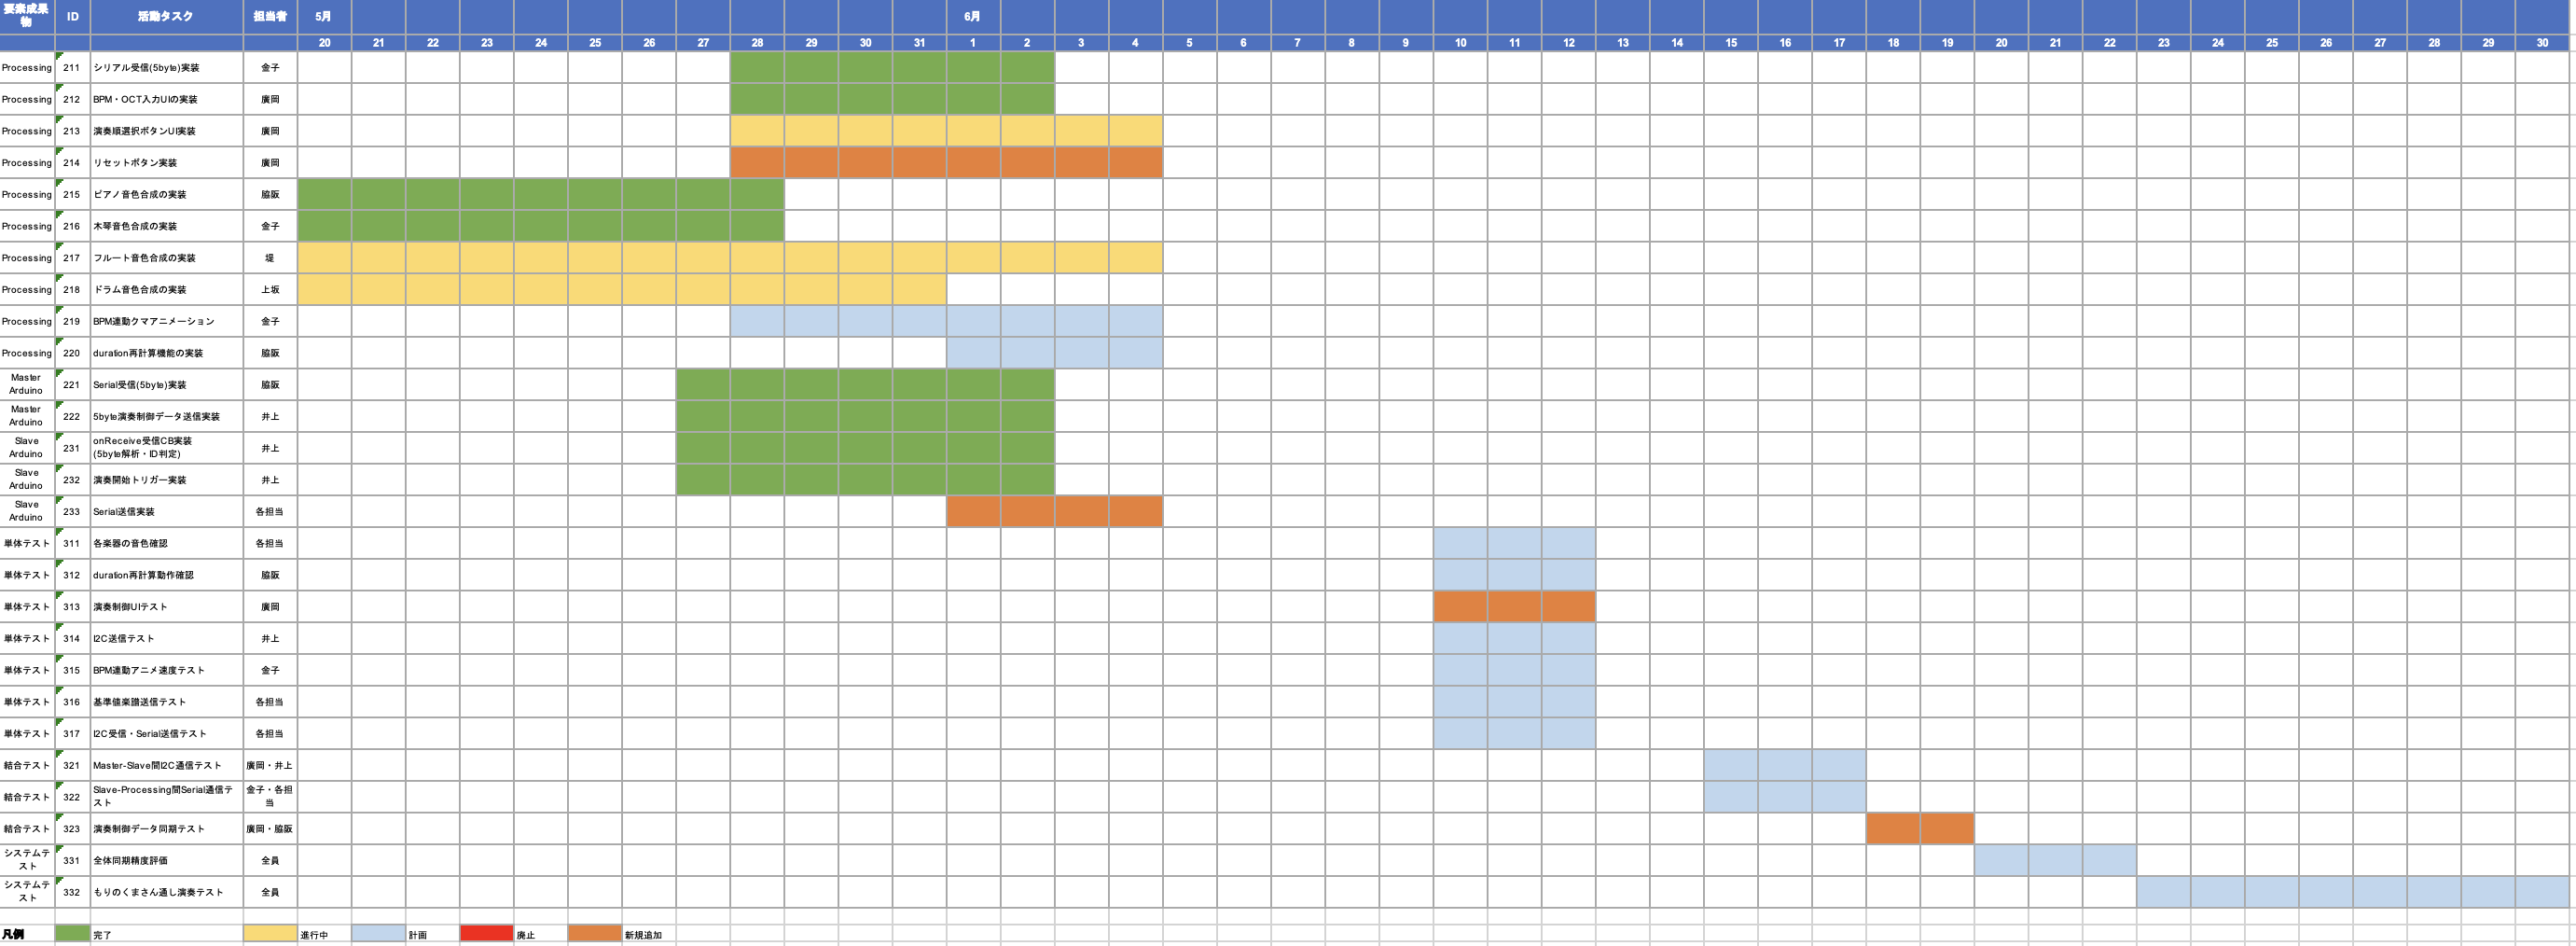
\includegraphics[width=13cm]{./figs/GC.png}
\caption{計画書より引用した，計画時点でのGC}
\label{GC1}
\end{figure}

\begin{figure}[H]
\centering
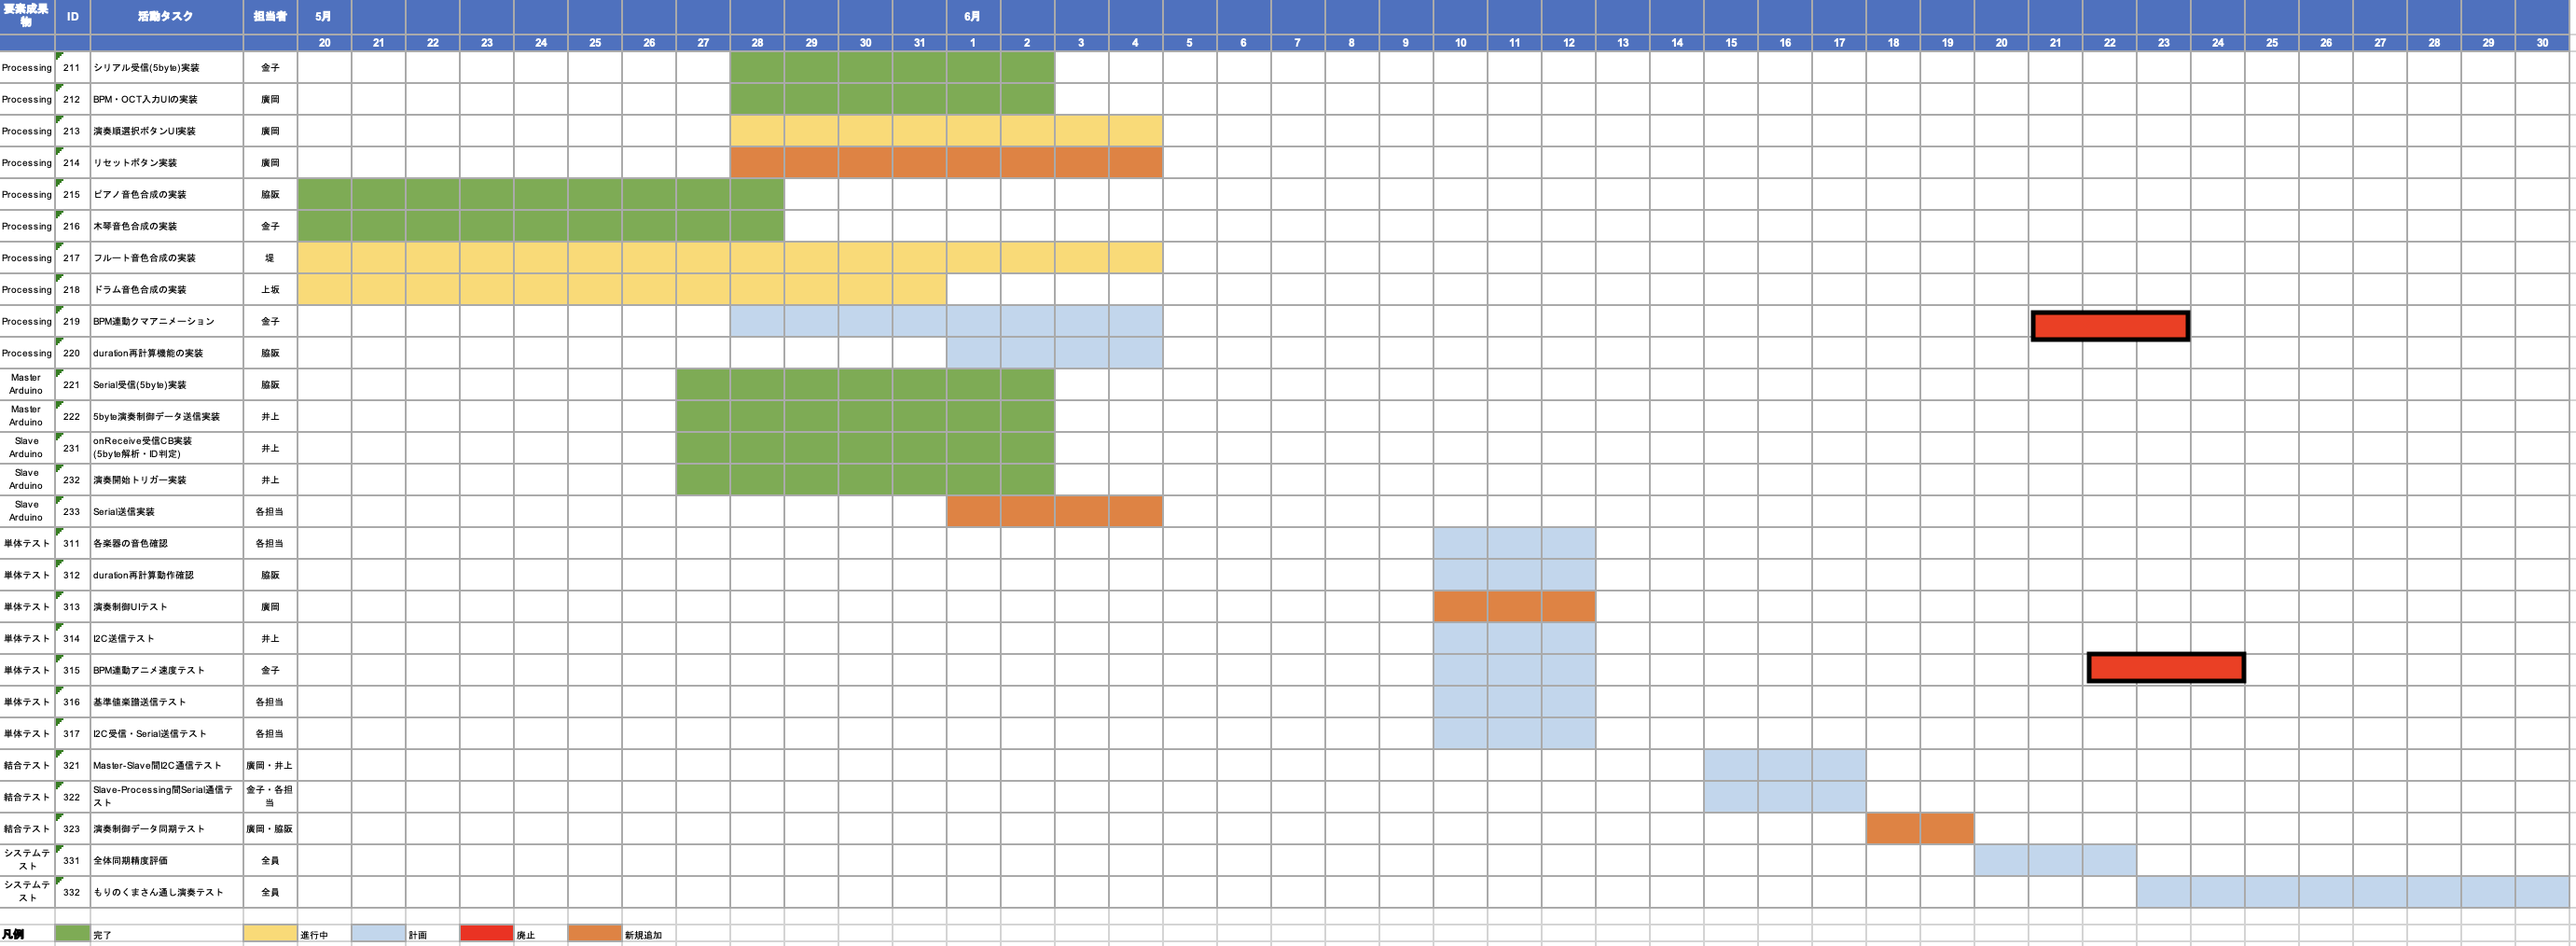
\includegraphics[width=13cm]{./figs/GC_now.png}
\caption{現在のGC（赤色：今週の進捗）}
\label{GC2}
\end{figure}

今週は全体結合テストの成功によりTRL 4への到達を果たした．
また，楽譜仕様変更への対応として関連5ファイルを更新し，新フォーマットへの移行が完了した．
残課題は中級楽譜の実データ受領と輪唱オフセット値の再調整であり，次週の対応を予定している．


\begin{thebibliography}{99}

\bibitem{font_fix}
  codeaid，Processing で日本語を表示する方法，
  \url{https://codeaid.jp/processing-jp/}，
  2026年6月26日参照．

\bibitem{wire_lib}
  Arduino，Wire Library，Arduino Reference，
  \url{https://docs.arduino.cc/language-reference/en/functions/communication/wire/}，
  2026年6月29日参照．

\bibitem{papplet_multiwin}
  Processing Foundation，\texttt{PApplet.runSketch()}，Processing Reference，
  \url{https://processing.org/reference/}，
  2026年6月22日参照．

\end{thebibliography}

\end{document}
